%TODO ewalds sphere, kohrenz->resolution

\documentclass[a4paper]{scrartcl}

\usepackage[utf8]{inputenc}
\usepackage[english]{babel}
\usepackage{lmodern} 
\usepackage[T1]{fontenc}
\usepackage{booktabs}
\usepackage{multirow}
\usepackage{wrapfig}


% PAKETE
\usepackage{siunitx}
\usepackage{graphicx}
\usepackage{placeins}
\usepackage{longtable}
\usepackage{enumitem}
\usepackage{bbm}
%\usepackage{sidecap}

\usepackage{amssymb} % math symbols
\usepackage{amsmath} % ams
\usepackage{amsfonts} % mathmatical fonts

% caption indenting
\usepackage[format=plain,indention=0em,labelfont=bf,margin=1em]{caption} 
\usepackage[protrusion=true,expansion=true]{microtype} % denser font, "-" behind line
\usepackage{esint} % nicer double and triple integrals
\usepackage{fancyhdr} % fancy headers
\usepackage[colorlinks=true,linkcolor=black,citecolor=black,filecolor=black,urlcolor=black]{hyperref}



% EINSTELLUNGEN
\sisetup{seperr,repeatunits=false}
\numberwithin{equation}{section}
\numberwithin{figure}{section}
\numberwithin{table}{section}

% EIGENE FUNKTIONEN
\newcommand{\re}{\operatorname{Re}}
\newcommand{\im}{\operatorname{Im}}
\newcommand{\gquote}[1]{\glqq #1 \grqq}

\newcommand{\eq}[2]{\begin{equation}#1\label{#2}\end{equation}}
\newcommand{\eqand}[0]{\hspace{.25cm} \bigwedge \hspace{.25cm}}
\newcommand{\grafik}[2]{\begin{figure}[h]\centering \includegraphics[width=10cm]{#1.eps}  \caption{#2} \label{#1} \end{figure} }
\newcommand{\grafikq}[3]{\begin{figure}[h]\centering \includegraphics[width=10cm]{#1.eps}  \caption[#2]{#3} \label{#1} \end{figure} }
\newcommand{\tbl}[3]{\begin{table}[h]\caption{#1}\label{#2}\begin{center}#3\end{center}\end{table}}
\newcommand{\Abbildung}[1]{\textsl{Abbildung \ref{#1}}}
\newcommand{\AbbildungI}[1]{\textsl{(Abbildung \ref{#1})}}
\newcommand{\Tabelle}[1]{\textsl{Tabelle \ref{#1}}}
\newcommand{\TabelleI}[1]{\textsl{(Tabelle \ref{#1})}}
\newcommand{\Formel}[1]{(\ref{#1})}
\renewcommand{\d}{\mathrm{d}}
\newcommand{\ve}[1]{\mathbf{ #1} }

\title{Ma 2: Low Energy Electron Diffraction (LEED) on Surfaces}
\subtitle{Tutor: Y. Kahn}
\author{Benjamin Huber, Carolin Wille}
\date{November 7, 2011}

\begin{document}
\thispagestyle{empty}
\maketitle
\tableofcontents
\clearpage


\section{Introduction}
Low energy electron diffraction (LEED) is a spectroscopic technique used to analyze the surface structure of a substrate. Its surface sensitivity results from the relatively small mean-free path length of the electrons, which depends on their energy and is determined by the so called universal curve shown in figure \ref{fig:uni}. For electrons of an energy below 200 eV the mean free path is less then 10 $\AA$, which is in the same order of magnitude as typical lattice constants of metals. The principles of LEED can only be understood within the framework of the wave-matter dualism, as the electron diffraction results in wave-like interference phenomena.


\begin{figure}
  \centering
   	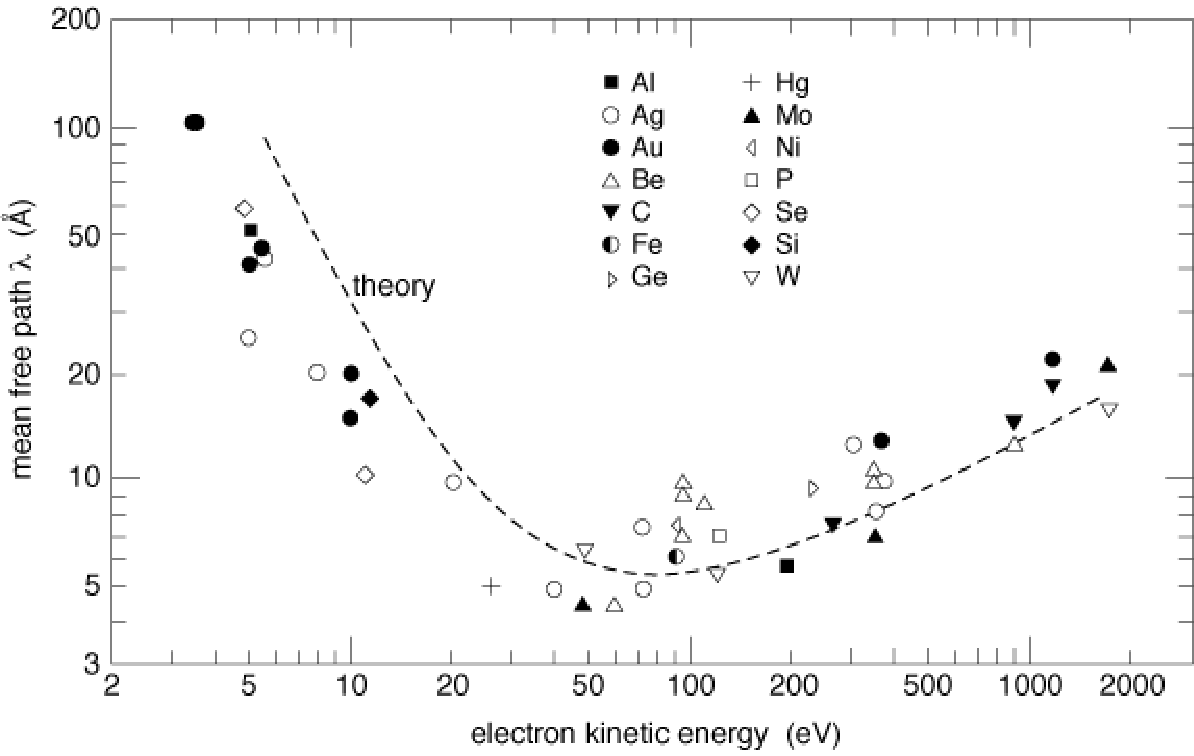
\includegraphics[width=0.5\linewidth]{pic/meanfree.pdf}

 \caption{\small Universal curve of solids \cite{zangwill}.  }
        \label{fig:uni}
\end{figure}
\FloatBarrier

\subsection{Matterwaves}
In 1924 de Broglie proposed, that any particle of momentum $p$ or mass $m$ and energy $E$ can be also described as a wave of wavelength 
\eq{\lambda = \frac{h}{p} =\frac{h}{2mE} \;,}{lambda}
where $h=4.136\times 10^{-15} \text{eVs}$ is the Planck constant. Therefore, electron scattering on surfaces can lead to intereference phenomena, if the electron wave length is of the order of the lattice constant. The de Broglie wave length of an electron, that is accelerated with a voltage $V_0$ is given by 
\eq{\lambda= \frac{\SI{12.26}{\AA}}{\sqrt{V_0}} \; }{lV}
and a typical eletron energy range from 50 to 500 eV corresponds to wavelengths between 0.5 and 2 $\AA$. Relativistic corrections have not to be taken into account in this energy range, as the ratio between velocity and speed of light for an electron accelerated with $V = \SI{500}{V}$ is given by
\eq{\frac{v}{c}=\sqrt{1-\frac{1}{(\frac{eV}{mc^2}+1)^2}} =0.04 \; .}{} 
and the relativistic correction given by the Lorentz factor $\gamma$ according to $\lambda_\text{rel.} = \frac{\lambda}{\gamma}$ is $\frac{1}{\gamma} = \sqrt{1-\frac{v^2}{c^2}}= 0.9992$. The acceleration for which relativistic effects would cause a deviation of $1\percent$ is given by
\eq{E=(\gamma -1)mc^2= \left(\frac{1}{0.99}-1\right)mc^2=\SI{5160}{eV}\;. }{}

\subsection{Constructive Interference for a surface scattering event}

Just as the Bragg Condition for constructive interference and the more advanced Laue theory are true for solid state physics these concepts can be applied to surface scattering as well. Analogue to the Bragg condition, the condition for constructive interference 
\eq{n \lambda = a_{h,k} (\sin \varphi - \sin \varphi_0 ) \;, \qquad n \in \mathbb N }{bragg}
can be derived from a simple geometrical consideration shown in figure \ref{fig:bragg}. The length $a$ is given by
\eq{a_{h,k} = |h \ve a_1 + k \ve a_2|\;, \qquad h,k \in \mathbb N \; , }{}
where $\ve a_1$ and $\ve a_2$ are the lattice vectors of the surface layer.
\begin{figure}
  \centering
   	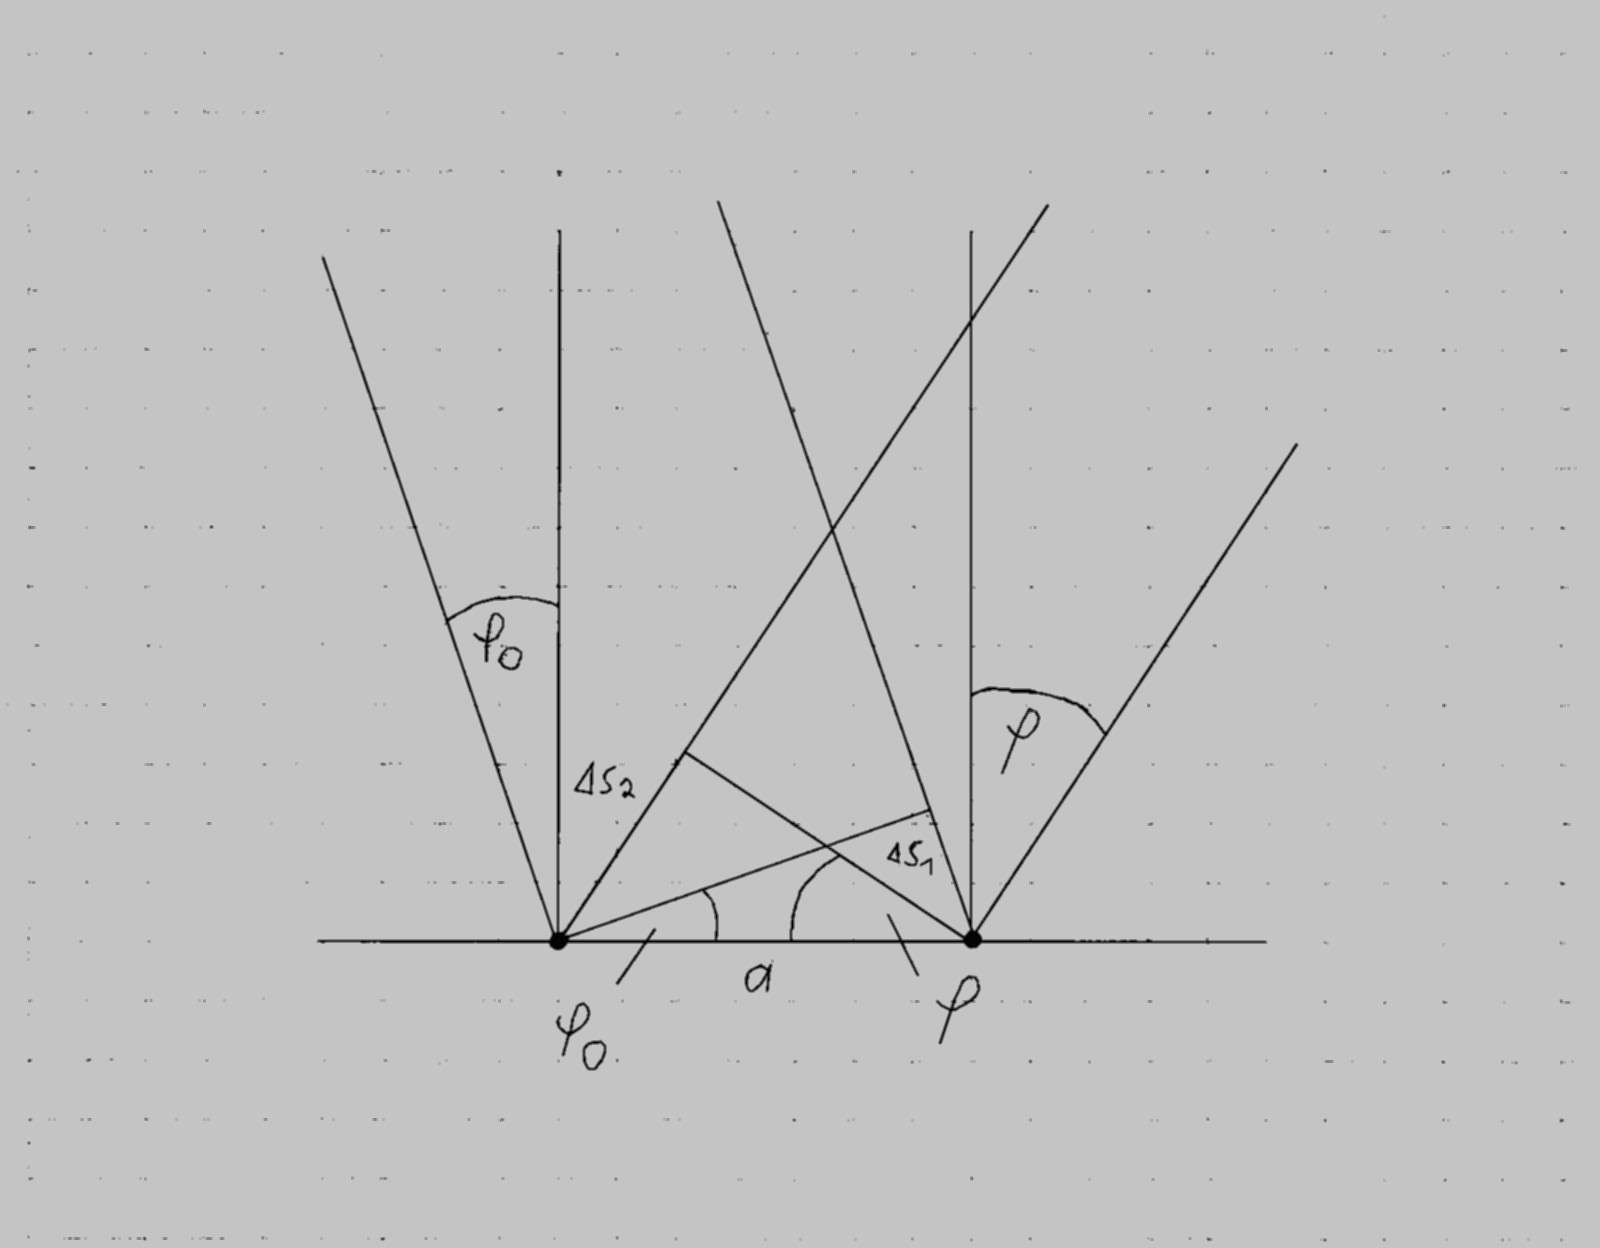
\includegraphics[width=0.5\linewidth]{pic/bragg.jpg}

 \caption{ Bragg-Reflexion on a Surface -- $\varphi_0$: angle of incoming wave, $\varphi$: angle of scattered wave. The optical path difference of the two wave fronts is given by $\Delta s_2 - \Delta s_1$.}
        \label{fig:bragg}
\end{figure}
\FloatBarrier

The scattering process can also be described by the usage of the reciprocal lattice vectors $\ve a_{1,2}^* \perp \ve a_{2,1}$, constructed via
$a_{1,2}^*=\frac{1}{a_{1,2} \sin \gamma} $, $\gamma = \measuredangle \ve a_1, \ve a_2 $. Therefore, consider a wave function of a plane wave with wave vector $\ve k_0$, that is scattered at all atom positions $\ve R_i$ back to the direction of $\ve k$ 
\eq{\Psi \propto \sum_{i} f_i(\ve k_0, \ve k) e^{i(\ve k - \ve k_0) \cdot \ve R_i} \ ,}{}
where $f_i$ are the atomic structure factors. As $\ve R_i=h \ve a_1 + k \ve a_2$, the intensity of the wave $|\Psi|^2$ scattered by a lattice of $H \cdot K$ lattice points can be written as
\eq{I=|\Psi|^2 \propto |F|^2 \frac{\sin^2 \left( \tfrac 1 2 H \ve a_1 \cdot (\ve k - \ve k_0) \right)}{\sin^2 \left( \tfrac 1 2 \ve a_1 \cdot ( \ve k - \ve k_0 ) \right)} \cdot \frac{\sin^2 \left( \tfrac 1 2 K \ve a_2 \cdot (\ve k - \ve k_0) \right)} {\sin^2 \left( \tfrac 1 2 \ve a_2 \cdot ( \ve k - \ve k_0 ) \right)} \; , } {au}
where F is the structure factor of a unit cell. Expression \Formel{au} becomes  maximal for the condition
\eq{\ve a_1 \cdot (\ve k - \ve k_0) = h 2 \pi \qquad \vee \qquad \ve a_2 \cdot (\ve k - \ve k_0) = k 2 \pi \;.}{}
These two equations are fulfilled, whenever the vector $\ve k - \ve k_0$ is a reciprocal lattice vector
\eq{\ve g = 2 \pi (h \ve a_1^{*} + k \ve a_2^*) \; .}{}
The Laue conditions \Formel{au} can therefore be replaced by the condition
\eq{\ve k - \ve k_0 =\ve g_{h,k} \;.}{muh}
Grafically this condition can be represented by an ewalds sphere as seen in figure \ref{fig:ewald}.
\begin{figure}
  \centering
   	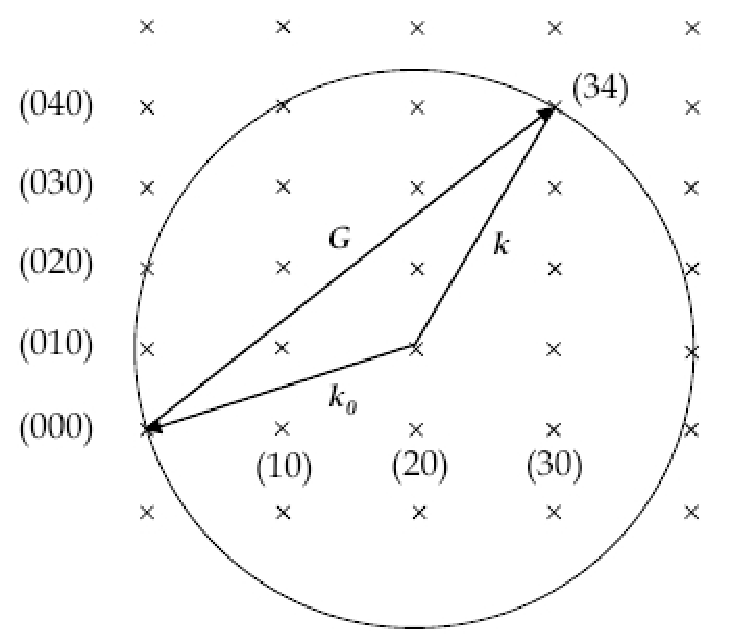
\includegraphics[width=0.5\linewidth]{pic/ewald.pdf}
 		\caption{ \small The ewalds sphere for a two dimensional quadratic lattice.  } %TODO beschreiben was k,k_0 und G sind.
      \label{fig:ewald}
\end{figure}
For an elastic scattering event, the absolute value of the wave-vector is conserved, i.e. $|\ve k|=|\ve k_0|$ and condition \Formel{muh} reduces to
\eq{2\ve k \cdot \ve g_{h,k} = g_{h,k}^2 \; .}{}
In three dimension, it is easy to show, that inserting the definition of the wave vector $\ve k=\frac{2\pi}{\lambda} \ve s$ and using the fact that $|\ve g_{h,k,l}| = 1/a_{h,k,l}$, we can rederive the Bragg condition. 

For two dimension another simple condition can be derived by multiplying the two Laue conditions \Formel{au} by $h$ and $k$, respectively and add them. Inserting the definition of the wave vector $\ve k=\frac{2\pi}{\lambda} \ve s$ yields
\eq{(\sin \varphi - \sin \varphi_0) |h \ve a_1 + k \ve a_2| = (h + k)^2 \lambda \; .} {}
This corresponds to a modified Bragg condition and can be simplified for perpendicular lattice vectors of the same length $a$ and a normal incoming wave, i. e. $\sin \varphi_0  =0$ to
\eq{\sin \varphi =\frac{\lambda}{a} \sqrt{h^2+k^2} \; .}{nm}

\subsection{Example for scattering laws in LEED}
Assuming a certain reflex characterized by $(h,k)$ of a copper surface, that has a quadratic lattice structure determined by $|\ve a_1|=|\ve a_2|=a=2.55 \AA$, shall be detected at an opening angle of $\varphi = 52 \degree$, what is the energy or the acceleration voltage of the scattering electron, that will create such a reflex?

Using formula \Formel{nm} and the relation between the de Broglie wave length and the energy of an electron \Formel{lV}, we obtain

\eq{ V =\frac{(12.26 \AA)^2}{a^2 \sin^2 \varphi} (h^2+k^2) = 37.23 (h^2 +k^2) \; .}{V}
\FloatBarrier
\begin{table}[!h]
\centering
\begin{tabular}{rr}
\toprule
Reflex $h$,$k$ & Energy (eV) \\
\midrule
1,0 & 37.23 \\
1,1 & 74.45 \\
2,2 & 297.80 \\
 \bottomrule
\end{tabular}
\caption{\small Values of electron energies for 3 specific reflexes at position $\varphi =52\degree$ calculated for a copper surface. }
\label{kll}
\end{table}

\begin{figure}
  \centering
   	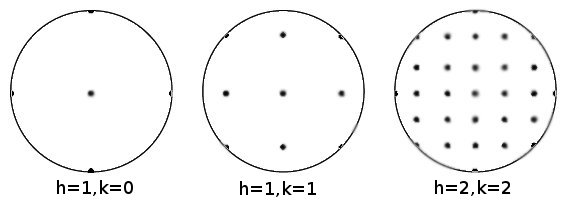
\includegraphics[width=0.7\linewidth]{pic/52.jpeg}

 \caption{\small Expected diffraction patterns for electron energies listed in table \ref{kll}.}
        \label{fig:bragg}
\end{figure}
\FloatBarrier


\subsection{Superstructures}
If the sample is unclean, it is likely, that the impurities will form a regular superstructure on the surface. As such they will contribute to the observed peaks. Figure \ref{fig:superstructure} is a sketch of a $(\sqrt{2} \times 2\sqrt{2})R45^\circ$ superstructure with the corresponding reciprocal lattice which would be observed in the case of such an impurity.
\begin{figure}[!bthp]
        \begin{center}
        \begin{tabular}{l r}
        		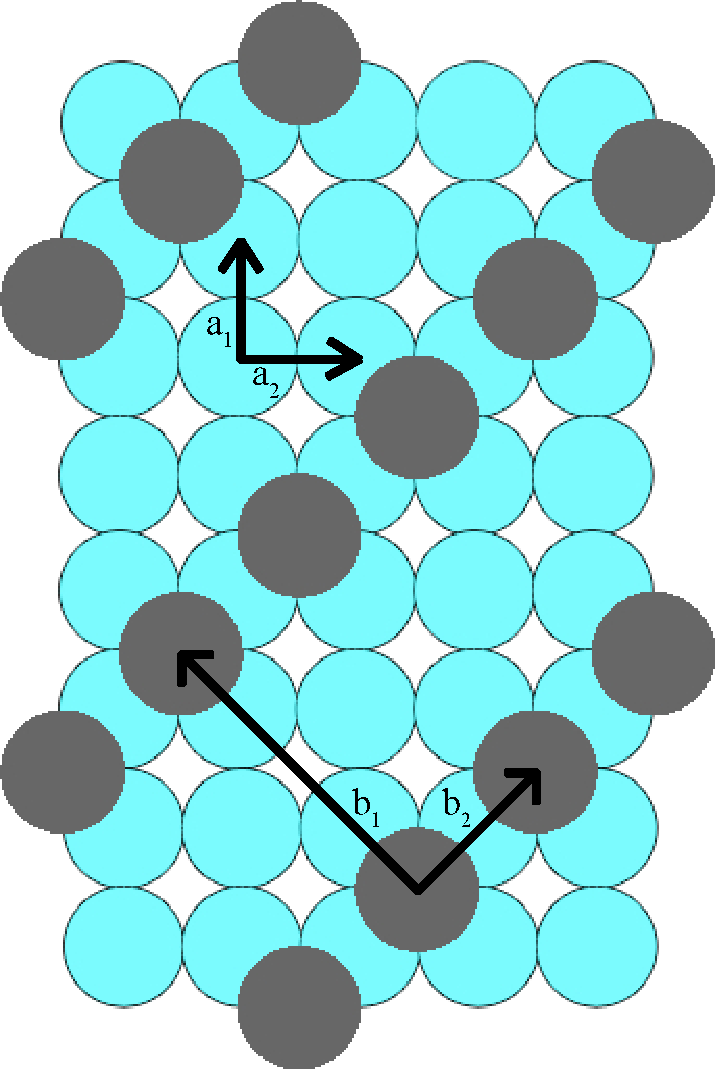
\includegraphics[width=0.2\linewidth]{pic/superstructure.pdf}
       	&
       		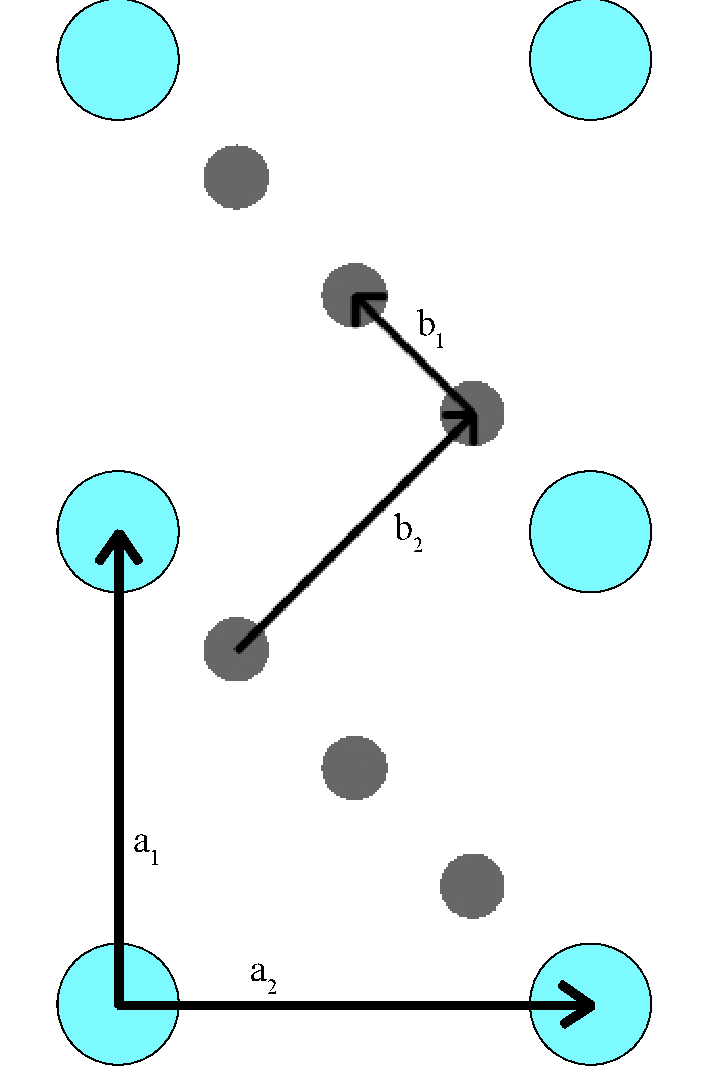
\includegraphics[width=0.2\linewidth]{pic/superstructure2.pdf}
		  \end{tabular}
        \end{center}
        \caption{
			\small \textbf{(left)} A regular square lattice (e.g. Cu atoms) with lattice vectors $a_{1,2}$ and a  $(\sqrt{2} \times 2\sqrt{2})R45^\circ$ superstructure with vectors $b_{1,2}$.
			\textbf{(right)} The same lattice in the reciprocal space.
        }
        \label{fig:superstructure}
\end{figure}


\subsection{Kinematic Approximation}
Disregarding the possible multiple scatterings of the electrons (the so called kinematic approximation) the reflection condition is the simple Bragg condition. Constructive interference occurs for length differences of $\Delta s = n\lambda$. Regarding only one a single beam (e.g. the (0,0) beam), the length difference is given by the lattice constants while the wavelength $\lambda$ is still variable (depending on the energy $V$). Measuring the intensity of this beam in dependence of the energy yields peaks whenever the difraction condition is met.

Taking into account the energy loss at the interface betweeen vacuum and matter $U$, the wavelength of the electrons is given by
\eq{\lambda = \frac{h}{2m\sqrt{V-U}}.}{}
Thus, the peaks in the $I(V)$ plot can be found at
\eq{V=\frac{h^2}{8md^2}n^2-U,}{}
where $d$ is the lattice constant.


\section{Experimental Set-Up and Measurement Procedures}

\subsection{Ultra High Vacuum (UHV)}
As the electrons used for spectroscopy easily interact with all kind of materials, it is very useful to operate in high vacuum. This is also necessary in order to reduce the rate of adsorption of molecules, which lead to disturbance of the measured spectra. (Ultra) high  vacuum (UHV) can only be achieved by a series of pumps acting within different pressure ranges. The four types used in the experiment are listed in table \ref{tab:pump}.
\begin{table}
\centering
\begin{tabular}{lr}
\toprule
pump & pressure range \\
\midrule
rotary vane pump & atm to $10^{-1}$ Pa \\ % todo atm -> Pa?
turbo molecular pump &  $1$ Pa to $10^{-9}$ Pa \\
ion getter pump  & $ 10^{-3}$ Pa to $10^{-9}$ Pa \\
titan sublimation pump & $10$ Pa to $10^{-9}$ Pa \\
\bottomrule
\end{tabular}
\caption{Different pumps and their pressure operating range.}
\label{tab:pump}
\end{table}

\subsubsection{Rotary vane pump}
The rotary vane pump is a simple mechanical pump, which consists of a cylinder connecting the vacuum cell and the outer space. In the cylinder a vane rotates and thereby shovels the gas to the outside. Springs ensure optimal contact between the vane and the cylinder walls. 

\begin{figure}
  \centering
   	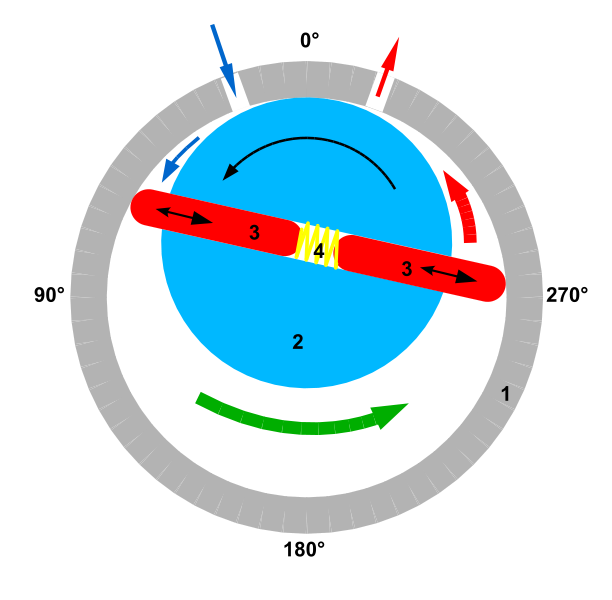
\includegraphics[width=0.3\linewidth]{pic/rot.png}

 \caption{\small Rotary vane pump. 1:pump housing, 2: rotor, 3: vanes, 4: spring}
        \label{fig:rot}
\end{figure}



\subsubsection{Turbomolecular pump}
The main features of a turbomolecular pump are the rotating blades (rotors), hitting the molecules very often per unit time, thereby enforcing a velocity distribution within the gas that is not isotropic, but a certain direction is preferred. Within the pump there are other static blades (stators), which act as a kind of filter to the velocity of the molecules in such a way, that molecules with the velocity, that is predominantly created by the rotors, can pass through with a higher probability. These filters act only in one-way, so that the molecules stay on the other side as long as the asymmetric velocity distribution is maintained. 
\begin{figure}
  \centering
  
   	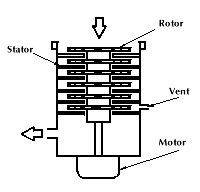
\includegraphics[width=0.3\linewidth]{pic/tu.jpg}

 \caption{\small Schematic description of a turbomolecular pump}
        \label{fig:turbo}
\end{figure}


\subsubsection{Ion getter pump}
In a ion getter pump high voltage is used to emit electrons an accelerate them. The electrons ionize molecules of the rest gas, which are then accelerated towards the surface, where they bind chemically. To lengthen the path of the electrons within the gas, a magnetic field is used to deflect the electrons thus creating a spiral like path. If a ion hits the electrode, several atoms are expelled and can build up a fresh layer on the other electrode. The material used for the electrodes is usually titan and it is often combined with a titan sublimation pump.

\subsubsection{Titan sublimation pump}
In a titan sublimation pump, titan is sputtered to create a fresh layer of atoms, which can absorb gases via chemical binding (chemisorption). In principle it is also possible to pump noble gas, which are inert, through simply catching them by covering them with a layer of titan. 

\subsection{Pressure Measurement}
For very low pressures usual manometers can't be used, because their are by are not sensitive enough. A manometer used for very low pressure is the ionization manometer, which can measure pressures as low as $10^{-8}$ Pa. It operates by emitting electrons from a thermal kathode and accelerating them towards the annode. Thereby the electron ionize the rest gas molecules, which are absorbed by the kathode leading to an ionization current, that is proportional to the pressure, but depends on the type of gas, as not all gases respond to ionizing electrons in the same way. An ionization manometer always has to be gauged.

\subsection{Sample Preparation}
To reduce the amount of impurities on the surface of the sample, several methods of cleaning are used. Apart from the purely mechanical removal by filing of the sample, sputtering is among the most commonly used. 

In sputtering, atoms of inert gases are accelerated towards the sample. Due to the kinetic energy surface atoms are blasted away leaving behind only the bulk of pure sample atoms.

As this is a rather random process, the surface is most likely very uneven after this process. To correct this, the sample is heated up to allow the atoms to reposition and form a smoother surface (tempering).

\subsection{Typical Set-Up}
A typical experimental set-up for LEED is shown in figure \ref{fig:leed}. Usually the electrons are shot at the probe under normal angle and the back scattered electrons are detected on a spherical fluorescence screen. In front of the screen is a system of spherical grids deflecting the electrons. The first grid is grounded to prevent deflection of the scattered electrons, which could use to biased measurement data. To the second and third grid a voltage slightly smaller then the accelerating voltage is applied in order to potential barrier with finite width, that can't be passed by inelastically scattered electrons. The third grid is again grounded and the fluorescence screen is at a voltage accelerating the electrons which passed the 2nd and 3rd grid to the screen. On the screen the diffraction pattern can be viewed and via using a CCD camera, the intensities of the reflexes can also be analysed.

\begin{figure}
  \centering
   	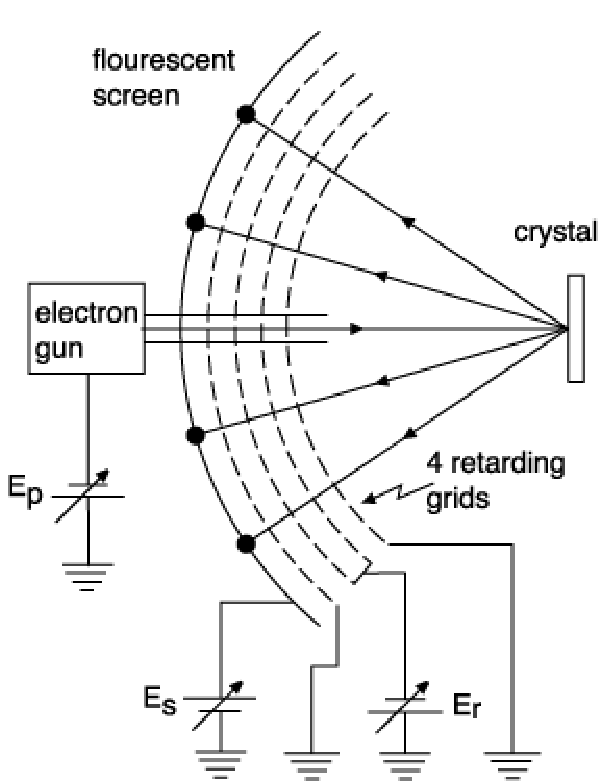
\includegraphics[width=0.3\linewidth]{pic/leed.pdf}

 \caption{\small Schematic Description of an LEED experiment. The retarding grits are used to select only elastically scattered electrons}
        \label{fig:leed}
\end{figure}


\subsection{Determination of Lattice Constant}
In order to determine the lattice constant of copper by analyzing the refraction pattern of the $(h,k)$ reflexes using equation \Formel{V}, first the opening angle of the spectrograph has to be determined. This is done by using the reflection of the $(0,0)$ beam, which vanishes from the screen at the angles $\Theta_L = 248.5 \degree$ and $\Theta_R=205.5 \degree$. The opening angle is therefore determined to be $\varphi=43 \degree$. 

The electron energy at which the reflex appears at the opening angle is measured and plotted against $(h^2+k^2)$. By linear regression the slope   of the line, that is proportional to $ 1/a^2 $  is determined. The voltage, were the reflex is at the opening angle is determined by the mean value of the voltage, where it is barely visible and the value, where it appears to be entirely visible. As this interval is closely correlated with the diameter of the reflexion peaks, half of this interval seems to be a reasonable error for the voltage or energy  values. For the $(1,0)$ peak, the energy could not be lowered sufficiently to apply this measuring methods, therefore it can only be set, that the energy needed to project this reflex onto the opening angle has to be below $\SI{47.7}{eV}$. All measurement values listed in table \ref{tab:reflexes} and are plotted in figure \ref{fig:reflexes}. Linear regression yields a slope $s=\SI{26.57(36)}{}$ which corresponds to a lattice constant 
\eq{a=\SI{3.65(3)}{\AA}\;.}{a1}
\begin{table}
\centering
\begin{tabular}{rr}
\toprule
Energy (eV) & Reflex $h$, $k$ \\
\midrule
$< 47.7$ & $1, 0$ \\ 
$59.5 \pm 1.5$ &  $1, 1$\\
$114.4 \pm 3.2$  & $2, 0$\\
$134.2 \pm 4.1 $ & $2, 1$ \\
$219.4 \pm 2.3$ & $2, 2$ \\
$246.3 \pm 2.9 $& $3, 0$ \\
$(260.6 \pm 3.4$ & $3,1) $ \\
\bottomrule
\end{tabular}
\caption{\small Electron energies at which reflexes $(h,k)$ are projected to opening angle $\varphi=43 \degree$. The value in parentheses does not enter the evaluation as it seems to be too far off.}
\label{tab:reflexes}
\end{table}



 \bibliographystyle{unsrt}
\bibliography{FPbib}

\end{document}


